\subsection{On the brightness of stars with detected planets}
\begin{figure}[!t]
	\centering
	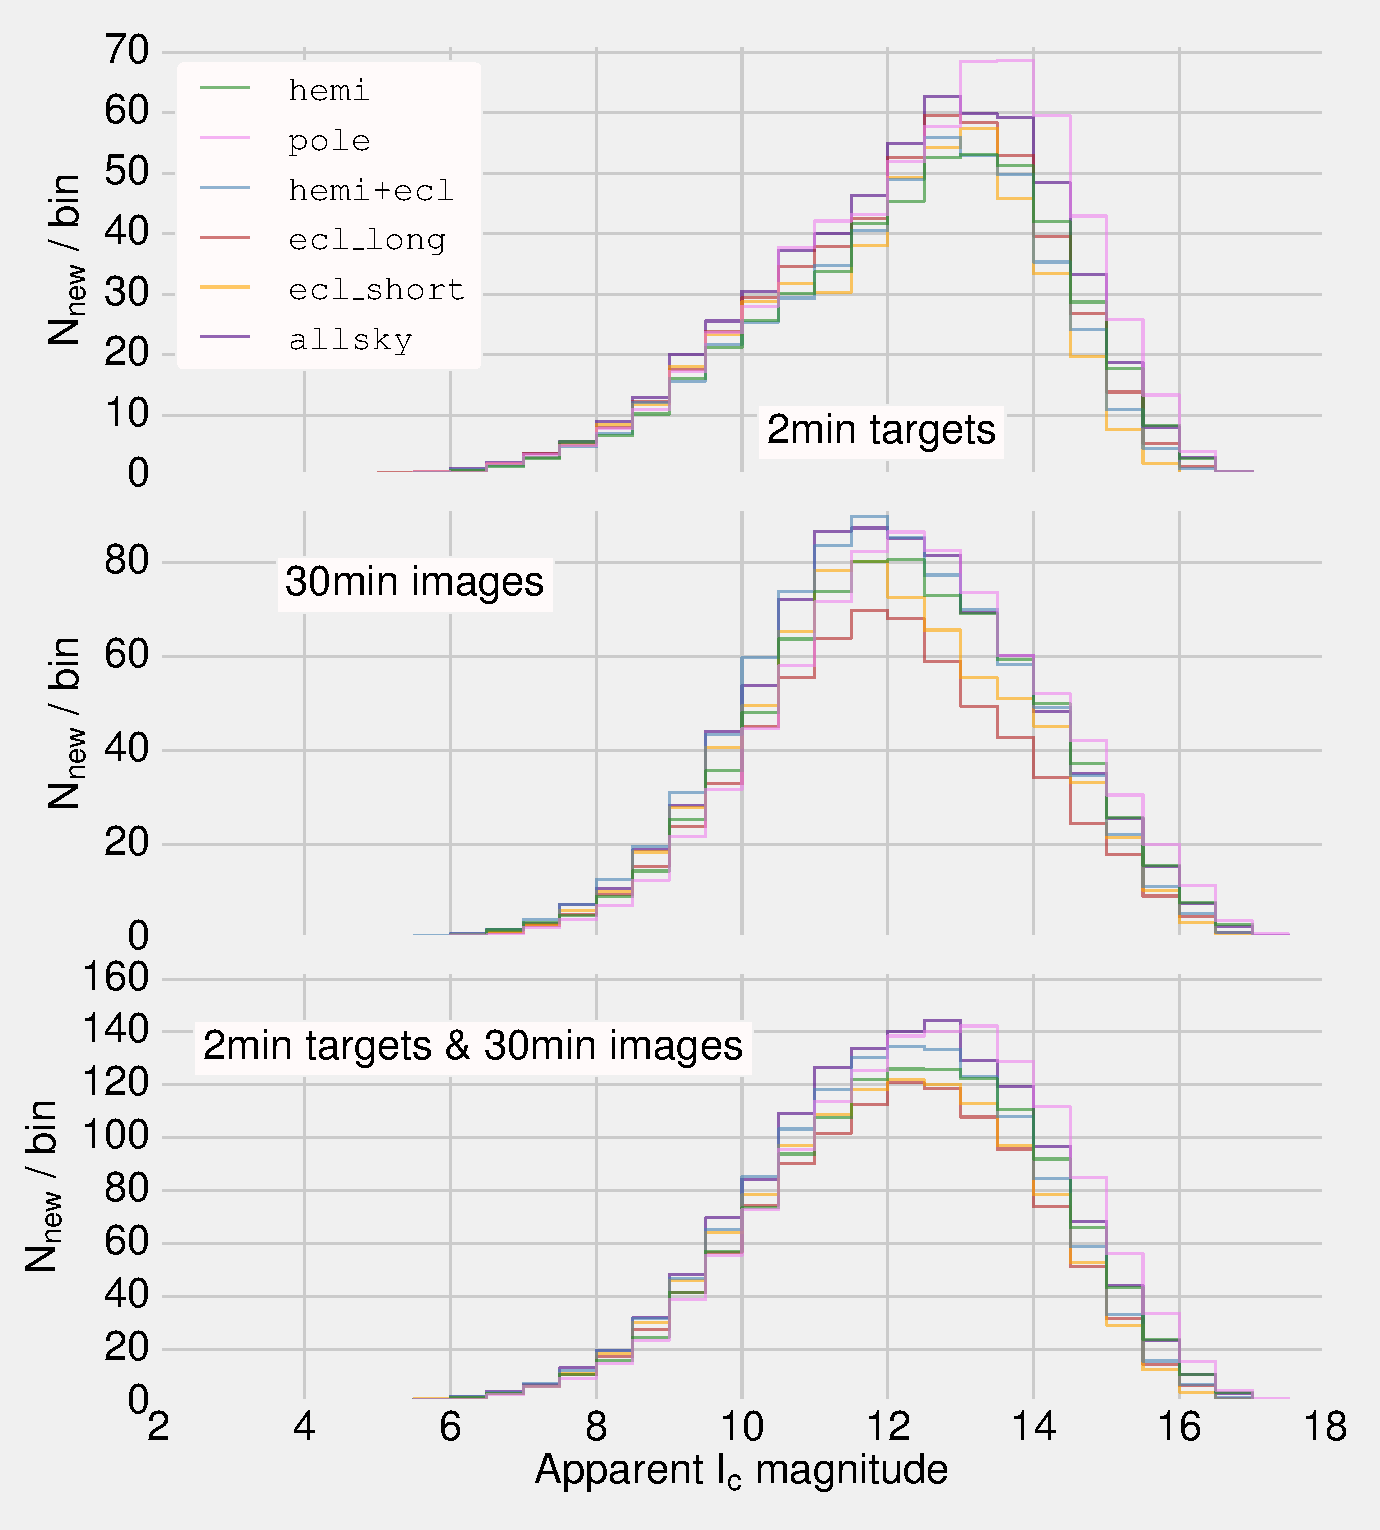
\includegraphics[]{figures/160729_icmag_t50_all.pdf}
	\caption{Histogram of apparent $I_c$ magnitude of host star for newly detected $R_p<4R_\oplus$ planets from all Extended Mission scenarios, for \textit{top:} postage stamp detections, \textit{middle:} full frame image detections, \textit{bottom:} the sums thereof.
	While \npole\ does well by most metrics, a larger proportion of the new planets it detects orbit dim stars compared to alternatives like \hemis\ or \shemiAvoid.}
	\label{fig:icmag_meta}
\end{figure}
While \npole\ does well by most metrics, a larger proportion of its newly detected planets orbit dim stars than the planet populations detected from alternatives like \hemis\ or \shemiAvoid.
We demonstrate this in Fig.~\ref{fig:icmag_meta}.
The main point here is that if in mission selection we were to assign extra weight towards detecting planets orbiting bright host stars, then \npole\ would do the worst.
% then why didn't we include this in fig 13?
For instance, arbitrarily setting the bound at $I_c<10$ and numerically integrating from Fig.~\ref{fig:icmag_meta}'s data, we see in Table.~\ref{tab:icmag_meta} that there is a $\sim30\%$ level difference between the missions.
For point of reference, the Primary Mission detects 386 such planets -- so a single year of Extended Mission detects roughly as many planets orbiting bright hosts as a single year of Primary Mission.
%cf bright_star_comparison_Ic_lt_10.ipynb
\begin{table}[!t]
	\centering
	\caption{Number of new, $I_c<10$, $R_p<4R_\oplus$ planets from each Extended Mission (average of 50 Monte Carlo realizations of our code; showing sum of PSs \& FFIs). \npole\ detects the fewest new planets orbiting bright stars.}
	\label{tab:icmag_meta}
	\begin{tabular}{|c|c|c|c|c|c|}
		\hline
		\nhemi & \npole & \shemiAvoid & \elong & \eshort & \hemis \\ \hline
		162    & 154    & 190         & 167    & 183     & 198    \\ \hline
	\end{tabular}
	%I put together this table by running /ext_mission_comparisons/memo_processing with the 160729_t50 data, and then just directly printing the numbers.
\end{table}

\begin{comment}
A related, but minor comment: \tesss is able to detect the smallest planets at the ecliptic poles, rather than near the ecliptic, due to background flux from zodiacal light. 

\begin{figure*}[th]
	\centering
	\todo[inline]{keep this figure? if so, make with 160729 data}
	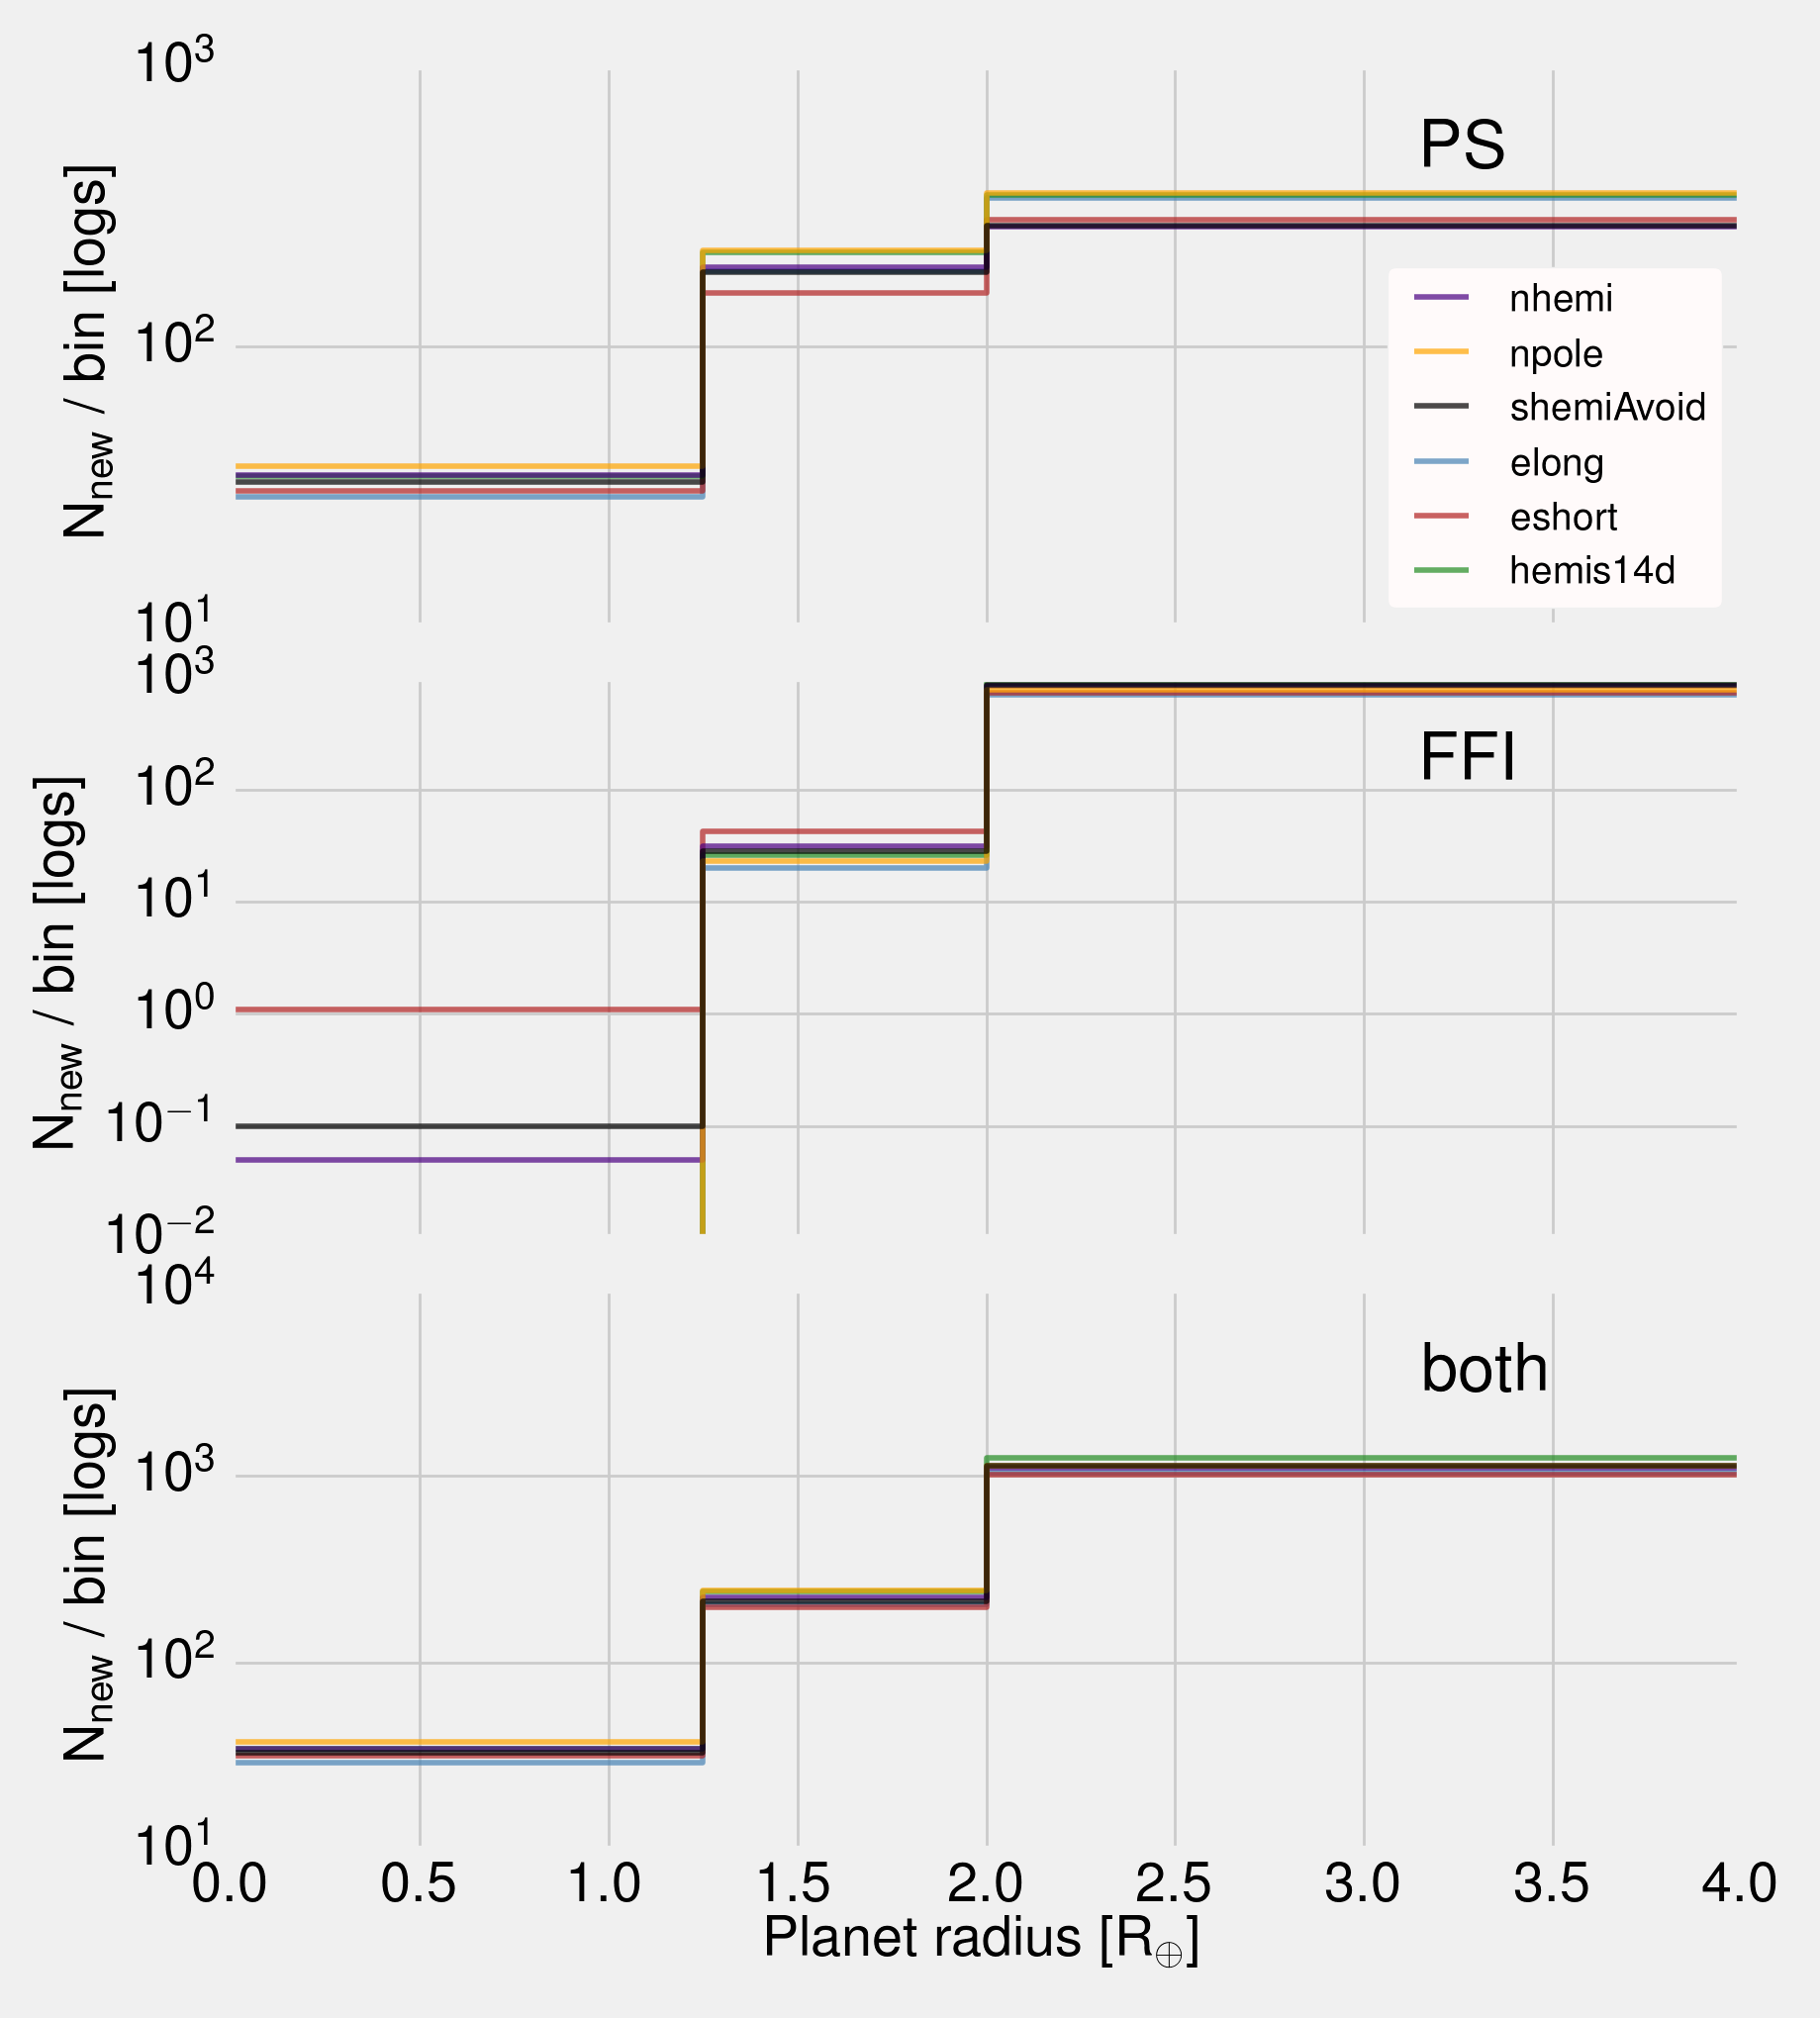
\includegraphics[]{figures/160708_r2_t20_all.png}
	\caption{\textit{Top:} words. \textit{Middle:} words. \textit{Bottom:} words.}
	\label{fig:r2_meta}
\end{figure*}
\end{comment}
